\cleardoublepage
\thispagestyle{empty}
\hbox{ }
\cleardoublepage

\appendix 

\section{INSERTANDO IMAGENES, TABLAS, CODIGO, ETC}

Im\'agenes:
\begin{figure}[h]
\centering
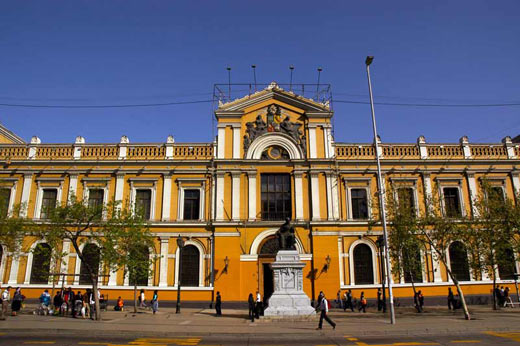
\includegraphics[scale=0.8]{figuras/uchile.jpg} 
\caption{\textsf{Universidad de Chile (escala 80\%)}}
\end{figure}

C\'odigo C, R, Java, etc:
\lstinputlisting{codigo/cargar-librerias.R}

\newpage

Tabla:

\begin{table}[h]
\centering
\begin{tabular}{l*{6}{c}r}
Variable              & Obs 1 & Obs 2 & Obs 3 & Obs 4 & Obs 5\\
\hline
V1 & 6 & 4 & 0 & 2 & 10 \\
V2            & 6 & 3 & 0 & 3 &  8 \\
V3           & 6 & 2 & 1 & 3 &  7 \\
V4     & 6 & 2 & 1 & 3 &  5 \\
\end{tabular}
    \caption{Tabla de ejemplo.}
\end{table}